\documentclass[11pt,a4paper]{article}
%\usepackage{fontspec, xunicode, xltxtra}  
%\setmainfont{Hiragino Sans GB}  
%\usepackage{xeCJK}
%\setCJKmainfont[BoldFont=STZhongsong, ItalicFont=STKaiti]{STSong}
%\setCJKsansfont[BoldFont=STHeiti]{STXihei}
%\setCJKmonofont{STFangsong}

%使用Xelatex编译

% 设置页面
%==================================================
\linespread{2} %行距
% \usepackage[top=1in,bottom=1in,left=1.25in,right=1.25in]{geometry}
% \headsep=2cm
% \textwidth=16cm \textheight=24.2cm
%==================================================

% 其它需要使用的宏包
%==================================================
\usepackage[colorlinks,linkcolor=blue,anchorcolor=red,citecolor=green,urlcolor=blue]{hyperref} 
\usepackage{tabularx}
\usepackage{authblk}         % 作者信息
\usepackage{algorithm}     % 算法排版
\usepackage{amsmath}     % 数学符号与公式
\usepackage{amsfonts}     % 数学符号与字体
\usepackage{mathrsfs}      % 花体
\usepackage{amssymb}
\usepackage{bbm}
\usepackage{bbold}
\usepackage[framemethod=TikZ]{mdframed}

\usepackage{graphicx} 
\usepackage{graphics}
\usepackage{color}
\usepackage{xcolor}
\usepackage{tcolorbox}
\usepackage{lipsum}
\usepackage{empheq}

\usepackage{fancyhdr}       % 设置页眉页脚
\usepackage{fancyvrb}       % 抄录环境
\usepackage{float}              % 管理浮动体
\usepackage{geometry}     % 定制页面格式
\usepackage{hyperref}       % 为PDF文档创建超链接
\usepackage{lineno}          % 生成行号
\usepackage{listings}        % 插入程序源代码
\usepackage{multicol}       % 多栏排版
%\usepackage{natbib}         % 管理文献引用
\usepackage{rotating}       % 旋转文字,图形,表格
\usepackage{subfigure}    % 排版子图形
\usepackage{titlesec}       % 改变章节标题格式
\usepackage{moresize}   % 更多字体大小
\usepackage{anysize}
\usepackage{indentfirst}  % 首段缩进
\usepackage{booktabs}   % 使用\multicolumn
\usepackage{multirow}    % 使用\multirow

\usepackage{wrapfig}
\usepackage{titlesec}     % 改变标题样式
\usepackage{enumitem}
\usepackage{aas_macros}


\newcommand{\myvec}[1]%
   {\stackrel{\raisebox{-2pt}[0pt][0pt]{\small$\rightharpoonup$}}{#1}}  %矢量符号
\renewcommand{\vec}[1]{\boldsymbol{#1}}
\newcommand{\me}{\mathrm{e}}
\newcommand{\mi}{\mathrm{i}}
\newcommand{\dif}{\mathrm{d}}
\newcommand{\tabincell}[2]{\begin{tabular}{@{}#1@{}}#2\end{tabular}}

\def\kpc{{\rm kpc}}
\def\km{{\rm km}}
\def\cm{{\rm cm}}
\def\TeV{{\rm TeV}}
\def\GeV{{\rm GeV}}
\def\MeV{{\rm MeV}}
\def\GV{{\rm GV}}
\def\MV{{\rm MV}}
\def\yr{{\rm yr}}
\def\s{{\rm s}}
\def\ns{{\rm ns}}
\def\GHz{{\rm GHz}}
\def\muGs{{\rm \mu Gs}}
\def\arcsec{{\rm arcsec}}
\def\K{{\rm K}}
\def\microK{\mu{\rm K}}
\def\sr{{\rm sr}}
\newcolumntype{p}{D{,}{\pm}{-1}}

\renewcommand{\figurename}{Fig.}
\renewcommand{\tablename}{Tab.}

\renewcommand{\arraystretch}{1.5}

\setlength{\parindent}{0pt}  %取消每段开头的空格

\newcounter{theo}[section]\setcounter{theo}{0}
\renewcommand{\thetheo}{\arabic{section}.\arabic{theo}}
\newenvironment{theo}[2][]{%
\refstepcounter{theo}%
\ifstrempty{#1}%
{\mdfsetup{%
frametitle={%
\tikz[baseline=(current bounding box.east),outer sep=0pt]
\node[anchor=east,rectangle,fill=blue!20]
{\strut Theorem~\thetheo};}}
}%
{\mdfsetup{%
frametitle={%
\tikz[baseline=(current bounding box.east),outer sep=0pt]
\node[anchor=east,rectangle,fill=blue!20]
{\strut Theorem~\thetheo:~#1};}}%
}%
\mdfsetup{innertopmargin=10pt,linecolor=blue!20,%
linewidth=2pt,topline=true,%
frametitleaboveskip=\dimexpr-\ht\strutbox\relax
}
\begin{mdframed}[]\relax%
\label{#2}}{\end{mdframed}}

\newcommand*\widefbox[1]{\fbox{\hspace{2em}#1\hspace{2em}}}



\title{Vector Analysis}
\author{}
\date{\today}
\begin{document}

\maketitle
\cite{arfken}
\section{Coordinate transformations}
\subsection{Rotations}
\begin{align}
\mathbf{\hat{e}}_x = \cos \varphi \mathbf{\hat{e}}^\prime_x  - \sin \varphi \mathbf{\hat{e}}^\prime_y ~, \\ 
\mathbf{\hat{e}}_y = \sin \varphi \mathbf{\hat{e}}^\prime_x  - \cos \varphi \mathbf{\hat{e}}^\prime_y ~,
\end{align}
the unchanged vector $\vec{A}$ now takes the changed form
\begin{align}
\vec{A} &= A_x \mathbf{\hat{e}}_x + A_y \mathbf{\hat{e}}_y ~, \\
&= A_x (\cos \varphi \mathbf{\hat{e}}^\prime_x  - \sin \varphi \mathbf{\hat{e}}^\prime_y ) +A_y (\sin \varphi \mathbf{\hat{e}}^\prime_x  - \cos \varphi \mathbf{\hat{e}}^\prime_y) ~, \\
&= (A_x \cos \varphi +A_y\sin \varphi) \mathbf{\hat{e}}^\prime_x +(-A_x \sin \varphi +A_y \cos \varphi) \mathbf{\hat{e}}^\prime_y ~, \\
&= A^\prime_x \mathbf{\hat{e}}^\prime_x + A^\prime_y \mathbf{\hat{e}}^\prime_y ~, 
\end{align}
then
\begin{align}
& A^\prime_x = A_x \cos \varphi +A_y\sin \varphi ~, \\
& A^\prime_y = -A_x \sin \varphi +A_y \cos \varphi ~,
\end{align}
i.e.
\begin{equation}
\vec{A}^\prime = \renewcommand{\arraystretch}{0.7}
\begin{pmatrix}
A^\prime_x \\
A^\prime_y
\end{pmatrix} 
= \renewcommand{\arraystretch}{0.7}
\begin{pmatrix}
\cos \varphi & \sin \varphi \\
-\sin \varphi  & \cos \varphi 
\end{pmatrix} 
 \renewcommand{\arraystretch}{0.7}
\begin{pmatrix}
A_x \\
A_y
\end{pmatrix} 
\end{equation}
Suppose now starting from $\vec{A}$ as given by its components in the rotated system, $( A^\prime_x , A^\prime_y)$, and rotate the coordinate system back to its original orientation. This will entail a rotation in the amount $-\varphi$, 
\begin{equation}
\vec{A} = \renewcommand{\arraystretch}{0.7}
\begin{pmatrix}
A_x \\
A_y
\end{pmatrix} 
= \renewcommand{\arraystretch}{0.7}
\begin{pmatrix}
\cos (-\varphi) & \sin (-\varphi) \\
-\sin (-\varphi)  & \cos (-\varphi) 
\end{pmatrix} 
 \renewcommand{\arraystretch}{0.7}
\begin{pmatrix}
A^\prime_x \\
A^\prime_y
\end{pmatrix} 
= \renewcommand{\arraystretch}{0.7}
\begin{pmatrix}
\cos \varphi & -\sin \varphi \\
\sin \varphi  & \cos \varphi
\end{pmatrix} 
 \renewcommand{\arraystretch}{0.7}
\begin{pmatrix}
A^\prime_x \\
A^\prime_y
\end{pmatrix} 
\end{equation}
Let
\begin{equation}
\vec{S} = \renewcommand{\arraystretch}{0.7}
\begin{pmatrix}
\cos \varphi & \sin \varphi \\
-\sin \varphi  & \cos \varphi
\end{pmatrix} ~, ~~
\vec{S}^\prime = \renewcommand{\arraystretch}{0.7}
\begin{pmatrix}
\cos \varphi & -\sin \varphi \\
\sin \varphi  & \cos \varphi
\end{pmatrix} ~,
\end{equation}
then $\vec{S}^\prime = \vec{S}^{-1} $, $\vec{S}^\prime = \vec{S}^T$ and $\vec{S} \vec{S}^\prime = 1$. Since $\vec{S}$ is real, $\vec{S}^{-1} = \vec{S}^T$ means that it is \textcolor{red}{orthogonal}. The transformation connecting $\vec{A}$ and $\vec{A}^\prime$ (the same vector, but represented in the rotated coordinate system) is
\begin{align}
& \vec{A}^\prime = \vec{S} \vec{A} ~, \\
& \vec{A} = \vec{S}^\prime \vec{A}^\prime ~, \\
& \vec{A} = \vec{S}^\prime \vec{S} \vec{A} ~.
\end{align}
with $\vec{S}$ an orthogonal matrix.

\subsection{Orthogonal Transformations}
\begin{align}
\mathbf{\hat{e}}_x = (\mathbf{\hat{e}}^\prime_x \cdot \mathbf{\hat{e}}_x) \mathbf{\hat{e}}^\prime_x + (\mathbf{\hat{e}}^\prime_y \cdot \mathbf{\hat{e}}_x) \mathbf{\hat{e}}^\prime_y ~, \\ 
\mathbf{\hat{e}}_y = (\mathbf{\hat{e}}^\prime_x \cdot \mathbf{\hat{e}}_y) \mathbf{\hat{e}}^\prime_x + (\mathbf{\hat{e}}^\prime_y \cdot \mathbf{\hat{e}}_y) \mathbf{\hat{e}}^\prime_y ~, 
\end{align}
\begin{equation}
\vec{S} = \renewcommand{\arraystretch}{0.7}
\begin{pmatrix}
\mathbf{\hat{e}}^\prime_x \cdot \mathbf{\hat{e}}_x & \mathbf{\hat{e}}^\prime_x \cdot \mathbf{\hat{e}}_y\\
\mathbf{\hat{e}}^\prime_y \cdot \mathbf{\hat{e}}_x & \mathbf{\hat{e}}^\prime_y \cdot \mathbf{\hat{e}}_y
\end{pmatrix}
\end{equation}


The transformation from one orthogonal Cartesian coordinate system to another Cartesian system is described by an \textcolor{red}{orthogonal matrix}. An orthogonal matrix must have a determinant that is real and of magnitude unity, i.e., $\pm 1$. However, for rotations in ordinary space the value of the \textcolor{red}{determinant will always be $+1$}.

\subsection{Reflections}


\begin{equation}
\vec{S} = \renewcommand{\arraystretch}{0.7}
\begin{pmatrix}
-1 & 0 & 0 \\
0 & -1 & 0 \\
0 & 0 & -1
\end{pmatrix}
\end{equation}
which results in ${\rm det} S = -1$.
\begin{equation}
\vec{S} = \renewcommand{\arraystretch}{0.7}
\begin{pmatrix}
1 & 0 & 0 \\
0 & 1 & 0 \\
0 & 0 & -1
\end{pmatrix}
\end{equation}
which results in ${\rm det} S = -1$.

\subsection{Successive Operations}

\begin{equation}
\vec{A}^\prime = \vec{S}(R^\prime) \vec{S}(R) \vec{A} 
\end{equation}




\section{Rotations in $\mathbbm R^3$}

In $\mathbbm R^2$, all the elements of $\vec{S}$ depended on a \textcolor{orange}{single variable}, the rotation angle. In $\mathbbm R^3$, the number of independent variables needed to specify a general rotation is \textcolor{red}{three}: Two parameters (usually angles) are needed to specify the direction of $\mathbf{\hat{e}}^\prime_3$; then one angle is needed to specify the direction of $\mathbf{\hat{e}}^\prime_1$ in the plane perpendicular to $\mathbf{\hat{e}}^\prime_3$; at this point the orientation of $\mathbf{\hat{e}}^\prime_2$ is completely determined. Therefore, \textcolor{red}{of the nine elements of $\vec{S}$, only three are independent}. The usual parameters used to specify $\mathbbm R^3$ rotations are the \textcolor{red}{Euler angles}.

The Euler angles describe an $\mathbbm R^3$ rotation in three steps, the first two of which have the effect of \textcolor{blue}{fixing the orientation of the new $\mathbf{\hat{e}}^\prime_3$ axis} (the polar direction in spherical coordinates), while the third Euler angle indicates the \textcolor{blue}{amount of subsequent rotation about that axis}. The first two steps do more than identify a new polar direction; they describe rotations that cause the realignment. 


1. The coordinates are rotated about the $\mathbf{\hat{e}}_3$ axis counterclockwise (as viewed from positive $\mathbf{\hat{e}}_3$) through an angle $\alpha$ in the range $0 \leqslant \alpha < 2\pi$, into new axes denoted $\mathbf{\hat{e}}^\prime_1$, $\mathbf{\hat{e}}^\prime_2$, $\mathbf{\hat{e}}^\prime_3$. (The polar direction is not changed; the $\mathbf{\hat{e}}^\prime_3$ and $\mathbf{\hat{e}}_3$ axes coincide.)

2. The coordinates are rotated about the $\mathbf{\hat{e}}^\prime_2$ axis counterclockwise (as viewed from positive $\mathbf{\hat{e}}^\prime_2$) through an angle $\beta$ in the range $0 \leqslant \beta < 2\pi$, into new axes denoted $\mathbf{\hat{e}}^{\prime\prime}_1$, $\mathbf{\hat{e}}^{\prime\prime}_2$, $\mathbf{\hat{e}}^{\prime\prime}_3$. (This tilts the polar direction toward the $\mathbf{\hat{e}}^{\prime}_1$ direction; but leaves $\mathbf{\hat{e}}^{\prime}_2$ unchanged.)

3. The coordinates are now rotated about the $\mathbf{\hat{e}}^{\prime\prime}_3$ axis counterclockwise (as viewed from positive $\mathbf{\hat{e}}^{\prime\prime}_3$) through an angle $\gamma$ in the range $0 \leqslant \gamma < 2\pi$, into the final axes, denoted $\mathbf{\hat{e}}^{\prime\prime\prime}_1$, $\mathbf{\hat{e}}^{\prime\prime\prime}_2$, $\mathbf{\hat{e}}^{\prime\prime\prime}_3$. (This rotation leaves the polar direction, $\mathbf{\hat{e}}^{\prime\prime}_3$, unchanged.)

In terms of the usual spherical polar coordinates $(r, \theta, \varphi)$, the final polar axis is at the orientation $\theta = \beta, \varphi = \alpha$. The final orientations of the other axes depend on all three Euler angles.

\begin{equation}
\vec{S}_1(\alpha) = \renewcommand{\arraystretch}{0.7}
\begin{pmatrix}
\cos \alpha & \sin \alpha & 0 \\
-\sin \alpha & \cos \alpha & 0 \\
0 & 0 & 1
\end{pmatrix}
\end{equation}

\begin{equation}
\vec{S}_2(\beta) = \renewcommand{\arraystretch}{0.7}
\begin{pmatrix}
\cos \beta & 0 & -\sin \beta \\
0 & 1 & 0 \\
\sin \beta  & 0 & \cos \beta
\end{pmatrix}
\end{equation}

\begin{equation}
\vec{S}_3(\gamma) = \renewcommand{\arraystretch}{0.7}
\begin{pmatrix}
\cos \gamma & \sin \gamma & 0 \\
-\sin \gamma  & \cos \gamma & 0  \\
0 & 0 & 1
\end{pmatrix}
\end{equation}
%===========================================================================================================================
\begin{figure*}
\centering
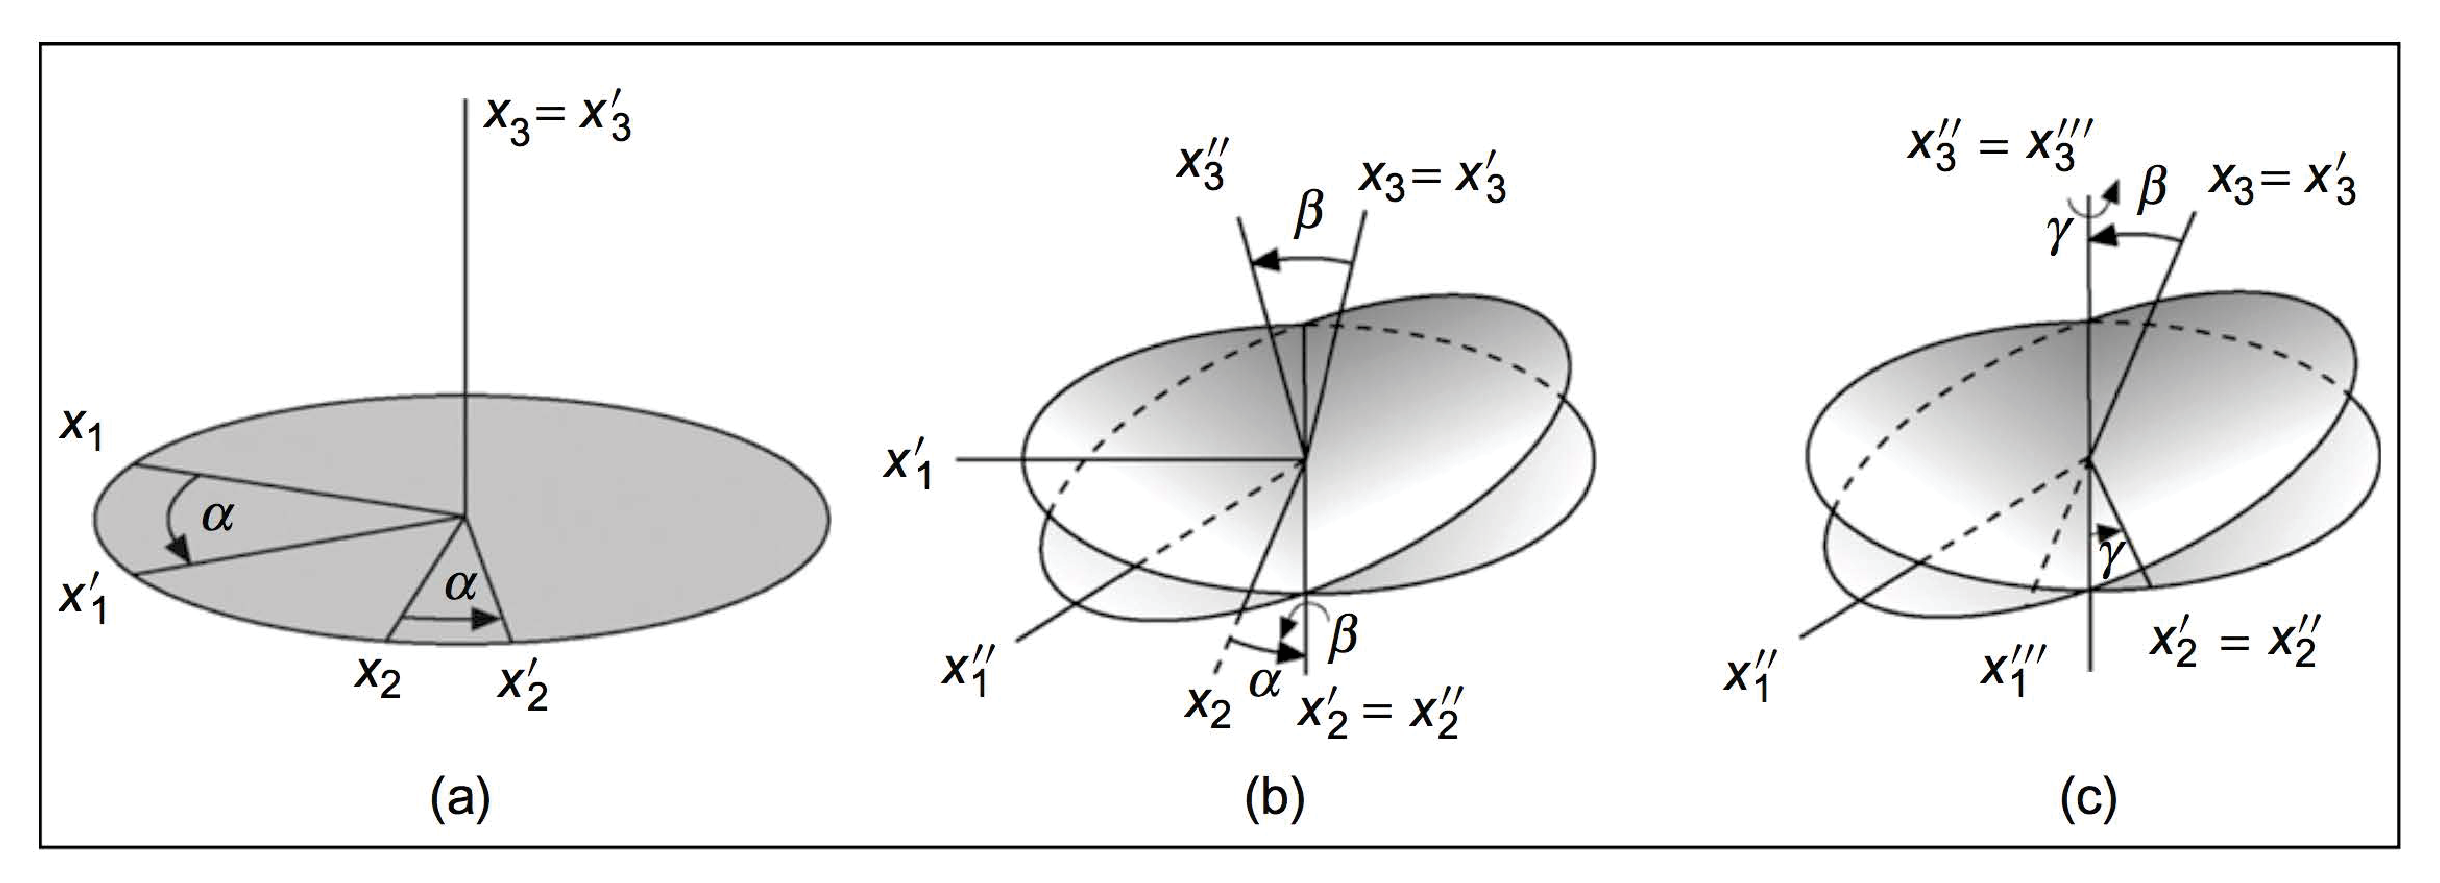
\includegraphics[height=5.cm, angle=0]{Euler_angle_rotations.eps}
\caption{
Euler angle rotations : (a) about $\mathbf{\hat{e}}_3$ through angle $\alpha$; (b) about $\mathbf{\hat{e}}^\prime_2$ through angle $\beta$; (c) about $\mathbf{\hat{e}}^{\prime\prime}_3$ through angle $\gamma$.
}
\label{fig:inlaplace}
\end{figure*}
%===========================================================================================================================
The total rotation is described by the triple matrix product
\begin{equation}
\vec{S}(\alpha, \beta, \gamma) = \vec{S}_3(\gamma) \vec{S}_2(\beta) \vec{S}_1(\alpha) ~,
\end{equation}
Note the order: $\vec{S}_1(\alpha)$ operates first, then $\vec{S}_2(\beta)$, and finally $\vec{S}_3(\gamma)$, i.e.
\begin{equation}
\vec{S}(\alpha, \beta, \gamma) = \renewcommand{\arraystretch}{0.7}
\begin{pmatrix}
\cos \gamma \cos \beta \cos \alpha -\sin \gamma \sin \alpha & \cos \gamma \cos \beta \sin \alpha +\sin \gamma \cos \alpha & -\cos \gamma \sin \beta \\
-\sin \gamma \cos \beta \cos \alpha -\cos \gamma \sin \alpha & -\sin \gamma \cos \beta \sin \alpha +\cos \gamma \cos \alpha & \sin \gamma \sin \beta \\
\sin \beta \cos \alpha & \sin \beta \sin \alpha & \cos \beta
\end{pmatrix}
\end{equation}
Each of $\vec{S}_1$, $\vec{S}_2$, and $\vec{S}_3$ are orthogonal, with determinant $+1$, so that the overall $\vec{S}$ will also be orthogonal with determinant $+1$.


\section{Curvilinear coordinates}




















%%%%%%%%%%%%%%%%%%%%%%%%%%%%%%%%%%%%%%%%%%%%%%%%%%%%%%%%%%%%%%%%%%%%%%
\bibliographystyle{unsrt_update}
\bibliography{ref}
%%%%%%%%%%%%%%%%%%%%%%%%%%%%%%%%%%%%%%%%%%%%%%%%%%%%%%%%%%%%%%%%%%%%%%

\end{document}